\section{Interest Flooding in NDN}
\label{sec:interest flooding}

% Points here:
% - Classification
% - Mechanisms: congestion and memory exhaustion
% - Target
% - Effectiveness: random names, non-existing content
% - Assumptions: the network, attackers, attack traffic, and legitimate consumers

%??? - References about other attacks and explicitly stating that this work aims to build a baseline for general Interest Flooding mitigation problem, with other attack profiles and malicious gateways.

\paragraph{Classification}

Interest flooding attack belongs to a class of network-level flooding attacks, where an attacker or a set of distributed attackers inject excessive amounts of Interests in order to overload the network and cause service disruptions for legitimate users (Fig.~\ref{fig:flooding example}).
%
% Definition of service
%
Service for legitimate users is disrupted when the network fails to satisfy Interests either because the Interests did not get through to (one of) the data producer(s) or nearby caches or the Data were lost on the way back (e.g., because of congested links).

\begin{figure}[htbp]
  \centering
  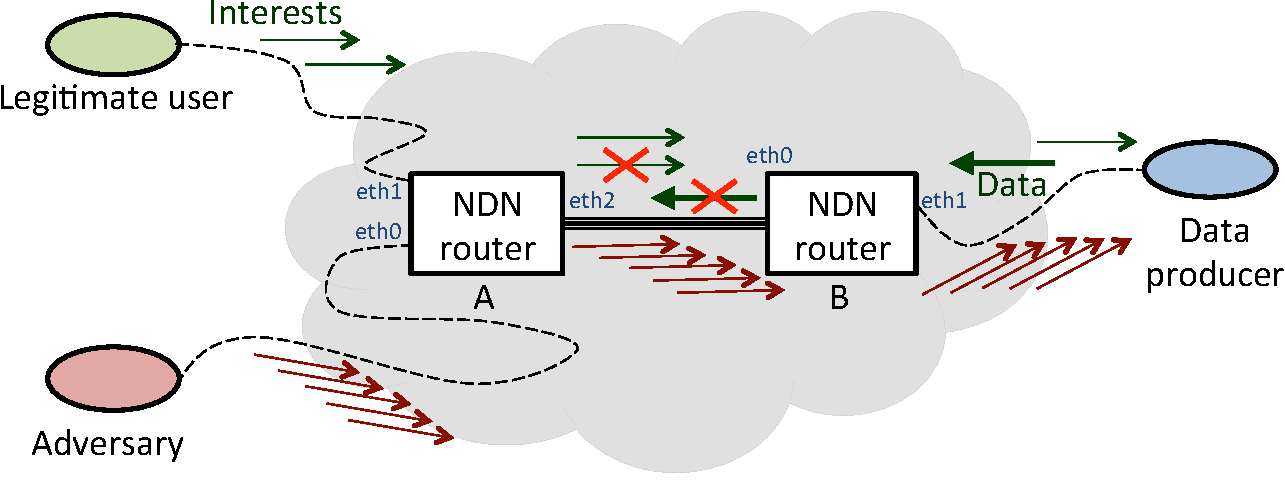
\includegraphics[width=\columnwidth]{attack-definition}
  \caption{Example of the Interest flooding attack}
  \label{fig:flooding example}
\end{figure}

\paragraph{Mechanism}

The Interest flooding attack has two-fold effect on service quality in NDN network: \textbf{creates network congestion} and \textbf{exhaust resources on routers}.

Like any other packets in the network, malicious Interests consume a portion network capacity.
Thus, a large amount of malicious Interests can lead to network congestion and drop of the legitimate Interests and Data packets.
%  (in case of bidirectional communication)
% The resource exhaustion effect can be much more ???.
% and more critical is the effect on memory and CPU resources of NDN routers.

As NDN routers maintain per-packet states for each forwarded Interest (entry in Pending Interests Table), an excessive volume of malicious Interests leads to creating an excessive number of PIT entries and exhaustion of routers' resources.
When a router has no memory to create a PIT entry for an incoming Interest, it drops this Interest.
% there is no point in forwarding the Interest further.
% Otherwise, if Data comes back, it would be considered unsolicited and dropped anyways.
Therefore, the routers' memory exhaustion effect may disrupt service for legitimate users even without causing network congestion.

\paragraph{Target}

Because communication in NDN is content-centric, it is impossible for an adversary to target specific routers or end-hosts, as neither of them have a global network identity.
However, an adversary can target a specific namespace, which in NDN network can loosely correspond to a network location or sets of network locations.
For example on Fig.~\ref{fig:flooding example}, if the Data producer is the exclusive owner of \ndnName{/foo/bar} namespace and is single-homed to router B, both router B and the Data producer would receive all Interests for \ndnName{/foo/bar/\ldots} that cannot be otherwise satisfied from in-network caches.
It should be noted that if connectivity in NDN network is rich (users are multi-homing to many providers, many interconnections between providers), targeting of specific locations is largely unfeasible, as stateful Interest forwarding strategy in NDN can fully and effectively utilize multiple available paths to destination~\cite{adaptive-forwarding}.

% \paragraph{Countermeasures}?

\paragraph{Effectiveness}
% Эффективность атаки
% - как можно повысить эффективность

% Effectiveness of the attack depends on how well volume of the Interests creates congestion near the Data producer, as well as how well r

Effectiveness of the Interest flooding attack directly depends on attack mechanism.

If the attack is primarily implemented using network congestion mechanism, then 

One of the key parameters for the effective Interest flooding attack is the way attackers generate names for the malicious Interests.
The stateful Interest forwarding and in-network data storage in NDN may nullify effect even of the large-scale flooding attack, if names for the malicious Interests are generated in a wrong way.
In particular, if distributed attackers generate similar names for the Interests, these Interests will be collapsed on NDN routers, resulting in a minuscule volume of the malicious Interests actually reaching the Data producer.
Also, if attackers express Interests for the data that can be returned from caches (popular Data or Data recently pulled by another attacker), the Data producer may not even receive any malicious Interest.

% Another parameter is how long Interests are sta

To implement an effective Interest flooding attack, one needs to ensure that a large volume of Interests is reaching targe 

Increase time Interests are staying on NDN routers.



NDN collapses similar Interests: attackers need to express different Interests in order to avoid collapsing
NDN caches data: attackers need to express junk Interests in order for interest to reach the data producer.



If malicious Interests can be collapsed or hit caches on the way towards to the Data producer, attack can have no effect at all.


the effect of the attack can be almost nullified. 

Lastl


Second factor is how well attack traffic is penetra

% How interest flooding attack can be the most effective
%

%Content Store (CS) is an effective obstacle for several types of DDoS attacks. CS possesses two important characteristics: maximum size and replacement policy. However, by knowing replacement policy attacker can construct a specific traffic generator that is using weaknesses of a chosen replacement procedure that will lead to increased processing time, slower packet delivery and in some cases de facto a complete inability to cache legitimate data. 


\paragraph{Assumptions}
% - assumptions about attacker position
% - assumptions about the producer / producer namespace
% - assumptions about the attack traffic / attack pattern

Not considering colluding attackers

% In this paper we are making an assumption that the attacker is trying to prevent legitimate users to access data from the producer by sending excessive amounts of Interests for data in the producers namespace, but which cannot be satisfied by the producer. 
% Assuming the network has only static content.  
% If the network having only static content, then there is no point for the attacker to issue satisfiable interests, as they I'll brig data, which will be cached nearby and future interests for the same name would not even reach vicinity of the producer. 
% That is, the effect of the attack will be minimized.
% Another point, that is probably is better. 
% If attacker issues interess that can be satisfied, then such interests will not stay in PITs long, not creating any challenges for the NDN routers' resources. 

% In this paper we are considering network level attacks performed by sending Interests with for non-existing data using prefix names with some random components. We make the assumption that the set of malicious clients (botnet) has a greedy behavior and tries to send as many false Interest packets as possible at any time given its connectivity options. Though NDN is capable of multipath Interest forwarding and forwarding strategy switching, we are using Best Route (single path) forwarding strategy in all of our experiments. 


\paragraph{Disclaimer}
In this paper we are not trying to completely solve all denial of service problems that can be caused by various variations of the Interest flooding attack.
Our primary focus is to demonstrate that while NDN opens door to new types of denial of service attacks, stateful packet forwarding in NDN makes it possible to mitigate such attacks, adding little additional complexity to the network.










%%% Local Variables: 
%%% mode: latex
%%% TeX-master: "paper"
%%% End: 
